\subsection{Energie}

\subsubsection{Recherchegrund}

Mit der Recherche über die Energie können wir abschätzen wie viel Energie gewonnen werden kann und welche Turbine dafür geeignet ist.

\subsubsection{Ergebnisse}

Um Energie aus fliessendem Wasser zu gewinnen gibt es drei unterschiedliche Möglichkeiten: Das Wasserrad, die Gleichdruckturbine und die Überdruckturbine. 

\paragraph{Wasserrad}
\begin{figure}[H]
	\centering
	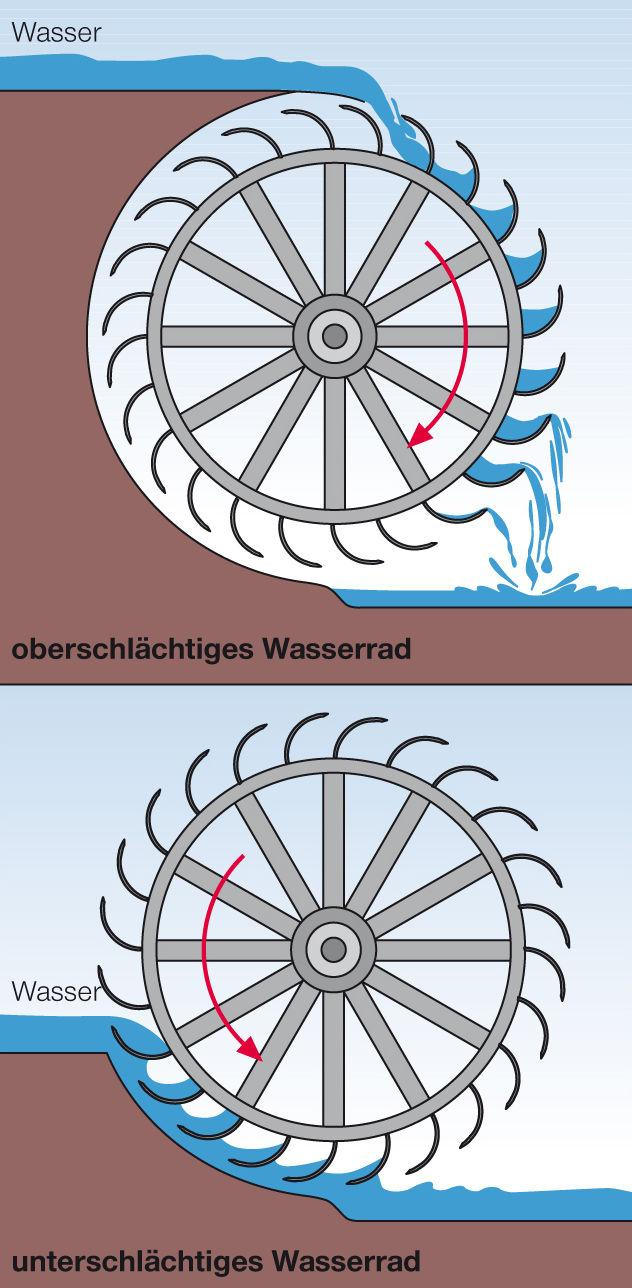
\includegraphics[width=4cm]{Wasserrad.jpg}
	\caption{Wasserrad \cite{wisse}} 
	\label{fig:Wasserrad}
\end{figure}

Das Wasserrad wird in fliessende Gewässer eingesetzt. Wie in der Abbildung \ref{fig:Wasserrad} \nameref{fig:Wasserrad} zu sehen fliesst das Wasser entweder von oben in die Schaufeln und das Rad beginnt sich durch das Gewicht des Wassers zu drehen, oder das Rad wird über dem Wasser platziert und das Rad bewegt sich durch den Fluss des Wassers.

\newpage

\paragraph{Überdruckturbine}
\begin{figure} [H]
	\centering
	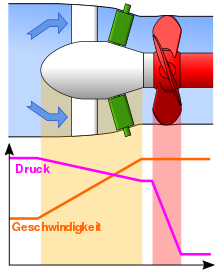
\includegraphics[width=4cm]{Ueberdruckturbine.png}
	\caption{Ueberdruckturbine \cite{wiki_ueberdruck}}
	\label{fig:Ueberdruckturbine}
\end{figure}

Bei der Überdruckturbine, zu sehen in der Abbildung \ref{fig:Ueberdruckturbine} \nameref{fig:Ueberdruckturbine}, sind die Schaufeln so ausgerichtet, dass sie beim Fluss des Wassers auf die Seite gedrückt werden und eine Drehbewegung resultiert. Dabei hat es vor den Schaufeln einen höheren Druck als hinter den Schaufeln

\paragraph{Gleichdruckturbine}
\begin{figure} [H]
	\centering
	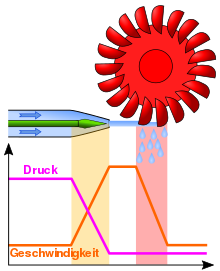
\includegraphics[width=5cm]{Gleichdruckturbine.png}
	\caption{Gleichdruckturbine \cite{wiki_gleichdruckturbine}}
	\label{fig:Gleichdruckturbine}
\end{figure}

In der Abbildung \ref{fig:Gleichdruckturbine} \nameref{fig:Gleichdruckturbine} ist eine Gleichdruckturbine zu sehen. Für die Turbine wird das Wasser von einer gewissen Höhe in einer Fallleitung nach unten befördert. Die potenzielle Energie des Wassers wird dabei in kinetische Energie umgewandelt und das Wasser trifft mit einer hohen Geschwindigkeit in den Turbinenraum. Um diese Energie zu nutzen wird nun der Wasserstrahl auf die Schaufeln der Pelton-Turbine gerichtet, die anschliessend zu drehen beginnt. 


\newpage

\paragraph{Entscheid}

Wir haben uns entschieden, dass eine Gleichdruckturbine (Pelton-Turbine) für unsere Anwendung am besten geeignet ist. Der grosse Vorteil der Pelton-Turbine ist, dass das Wasser keine enge Stelle durchqueren muss, wie dies bei einer Überdruckturbine der Fall wäre.Sie ist somit besser  vor Verstopfungen geschützt.

\paragraph{Berechnungen}

Die Endgeschwindigkeit des Wassers kann mit folgender Formel berechnet werden:
\begin{center}
\(v = \sqrt{2 \cdot g \cdot h} \)
\end{center}

Die Einheit der Geschwindigkeit \(v\) ist \si{m/s}, das Schwerefeld \(g\) auf der Erde besitzt den Wert 9.81~\si{N/kg}, und die Höhe \(h\) hat die Einheit \si{m}.

\bigskip

Die Energie, die gewonnen werden kann, wird mit folgender Formel berrechnet:

\begin{center}
\(E =\frac 12\ \cdot m \cdot v^2\)
\end{center}

Die Energie \(E\) hat die Einheit \si{J}, die Einheit der Geschwindigkeit \(v\) ist \si{m/s}, und die Masse \(m\) hat die Einheit \si{kg}

Um die Leistung zu erhalten, muss die Masse pro Zeit(1s) einberechnet werden. Die Masse wird  mit der Dichte und dem Volumenstrom ersetzt.

\begin{center}
\(P =\frac 12\ \cdot \varphi \cdot Q \cdot v^2\)
\end{center}

Die Leistung \(P\) hat die Einheit \si{W}, der Volumentstrom \(Q\) die Einheit \si{m^3/s}, die Dichte \(\varphi\)  \si{kg/m^3} und die Geschwindigkeit \(v\)  \si{m/s}.

\bigskip


Mit diesen physikalischen Grundlagen kann nun die Leistung in Abhängigkeit der Höhe und des Volumenstromes berechnet werden.  Die Berechnungen sind in der Tabelle  \ref{tab:Leistungsberechnung} \nameref{tab:Leistungsberechnung} ersichtlich.

\begin{table} [H]
	\centering
	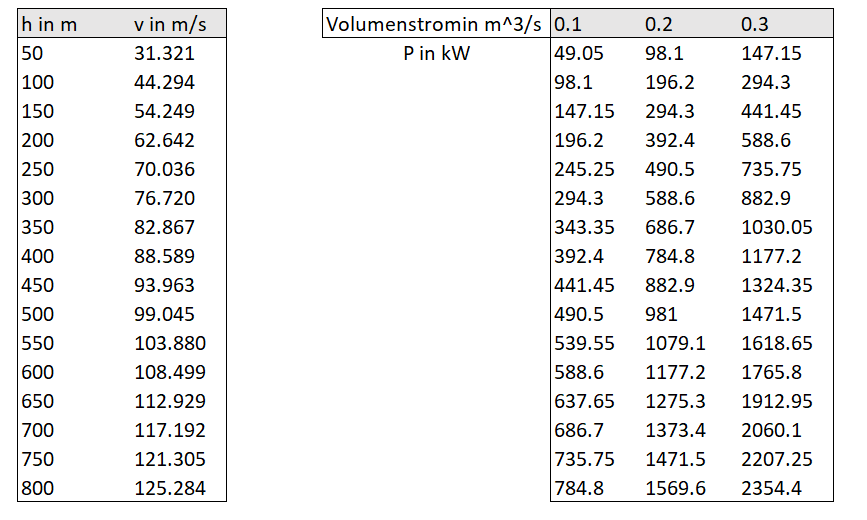
\includegraphics[width=13cm]{Leistungsberechnung.png}
	\caption{Leistungsberechnung}
	\label{tab:Leistungsberechnung}
\end{table}

\newpage

Dies ist nur die theoretische Leistung. Mit der Reibung am Rohr und dem Widerstand der Luftsäule wird das Wasser stark abgebremst. Gemäss dem Informationszentrum Entwässerungstechnik Guss e.V. (IZEG), die Versuche mit der Fallgeschwindigkeit durchgeführt haben, wird das Wasser bereits nach 15\si{m} nicht mehr mehrklich schneller. Dies ist in der Abbildung \ref{fig:Fallgeschwindigkeit} \nameref{fig:Fallgeschwindigkeit} gut ersichtlich.

\begin{figure} [H]
	\centering
	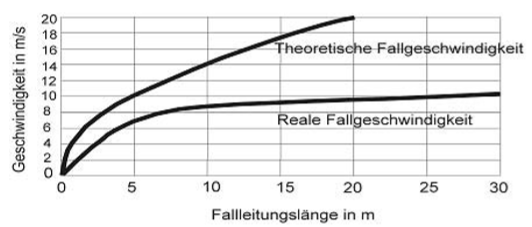
\includegraphics[width=10cm]{Fallgeschwindigkeit.png}
	\caption{Fallgeschwindigkeit \cite{Izeg}}
	\label{fig:Fallgeschwindigkeit}
\end{figure}


Mit der Endgeschwindigkeit von 10 \si{m/s} wird bei einem Volumenstrom von 0.1 \si{m^3/s} noch 5 \si{kW} erzeugt.

\subsubsection{Fazit}

Die gewonnene Leistung nimmt ab ca. 15\si{m} nicht mehr merklich zu. Der Grundgedanke, dass die Geschwindigkeit des Wassers in grossen Fallhöhen zunimmt, funktioniert nur, wenn die Fallleitung komplett mit Wasser befüllt wäre und somit der Luftwiderstand wegfällt.

Damit man mit diesem System trotzdem Energie zurückgewinnen kann, müsste alle 15\si{m} eine Turbine die Energie des Wassers umwandeln.

\clearpage 





